\documentclass[fr]{../../../../../../eplexam}

\usepackage{../../../../../../eplunits}

\graphicspath{{img/}}

\hypertitle[']{Optique et lasers}{7}{PHYS}{2143}{2019}{Janvier}{All}
{Martin Braquet \and Olivier Leblanc}
{Alain Cornet, Baptiste Fabre et Clément Lauzin}

Examen de 4h à 4 questions, où on demande de choisir seulement 3 questions auxquelles répondre.
Un formulaire manuscrit recto-verso format A4 est autorisé.

\section{Équation différentielle des rayons dans un milieu inhomogène}

\subsection*{Partie I}

Contexte : Nous voulons étudier l'existence de mirages. Dans un désert chaud, l'indice de réfraction varie avec la hauteur selon une loi :

\[
    n^2(z) = az+b
\]

On pose K tel que : $n_0 \sin(i_0) = \frac{1}{\sqrt{K}}$.

\begin{figure}[h!]
    \centering
    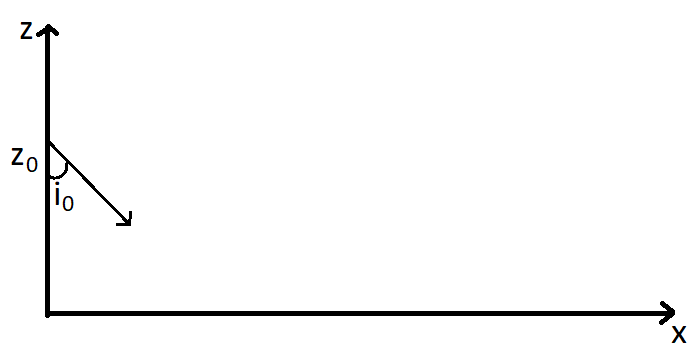
\includegraphics[scale=0.6]{02.png}
    \caption{}
    \label{}
\end{figure}

\begin{enumerate}
 \item Rappeler l'équation différentielle des rayons lumineux.
 \item Montrer que la trajectoire peut s'écrire :
    \[
    z = \frac{aK}{4} x^2 + \frac{\cos(i_0)}{\sin(i_0) x + z_0}
    \]
 \item Expliquer la forme de la trajectoire. Quelle est sa concavité ?
 \item Justifier l'existence des mirages en s'aidant d'un schéma.
\end{enumerate}

\subsection*{Partie II}

On désire former un rayon lumineux qui se propage entre deux plans horizontaux espacés d'une hauteur a selon une loi sinusoïdale : $ z = \mathrm{asin}(bx) $.

Montrez que l'expression de l'indice de réfraction du milieu (ne dépendant que de z) peut s'écrire : 
\[
    n(z) = n_0 \sqrt{1 - \frac{b^2}{1+a^2b^2}z^2}
\]


\begin{solution}
 
 \subsection*{Partie I}
 
 \begin{enumerate}
  \item \begin{center}
            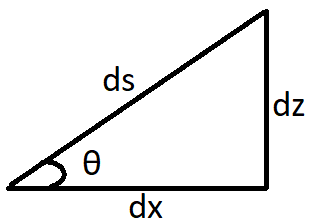
\includegraphics[scale=0.3]{01.png}
        \end{center}

    La loi de Snell-Descartes donne : $$n_0\sin(i_0) = \frac{1}{\sqrt{K}} = n(z) \cos(\theta)$$
    De plus, on a : 
    \[
        \sin(\theta)^2 + \cos(\theta)^2 = 1 \Leftrightarrow \cos(\theta) = \frac{1}{\sqrt{1+\tan(\theta)^2}} = \frac{1}{\sqrt{1+(\frac{dz}{dx})^2}}
    \]

    Donc, l'équation différentielle des rayons est : 

    \[
        \frac{1}{\sqrt{K}} = \frac{n(z)}{\sqrt{1+(\frac{dz}{dx})^2}}
    \]
  \item On intègre l'équation différentielle en tenant compte de l'expression donnée de $n(z)$ : 
    \[
        \frac{1}{\sqrt{K}} = \frac{n(z)}{\sqrt{1+(\frac{dz}{dx})^2}}  \Leftrightarrow (aK)z+(bK) = 1 + (\frac{dz}{dx})^2  \Leftrightarrow \left[(aK)z + (bK-1)\right]^{\frac{-1}{2}} dz = dx
    \]
    \[
        \Leftrightarrow \frac{2[(aK)z + (bK-1)]^{\frac{1}{2}}}{(aK)} = x + C
    \]
    \[
    \Leftrightarrow (aK)z + (bK-1) = \left( \frac{(aK)x}{2} + C' \right) ^2 = \frac{(aK)^2}{4}x^2 + (aK)C'x + C'^2 \Leftrightarrow z = \frac{(aK)}{4} x^2 + C'x + z_0 
    \]

    Avec la condition limite : $ \frac{dz}{dx} (x=0) = \frac{1}{\tan(i_0)} = C'$ (voir dessin), on retombe sur l'expression de l'énoncé.
  \item La trajectoire est une parabole orientée vers le haut (car $\frac{(aK)}{4}$ est positif).
  \item Puisque la lumière subit une trajectoire courbée, les rayons lumineux changent de direction à l'approche du sol (chaud) pour ainsi repartir vers le haut. Une personne interceptant ces rayons lumineux qui remontent va alors voir les couleurs bleutées du ciel alors que l'axe de ses yeux est dirigé vers le sol. De cette manière, la personne interprète cette couleur bleue par un lac alors qu'il s'agit du ciel.
 \end{enumerate}
 
 \subsection*{Partie II}

Comme on impose $z = a \sin(bx)$, il faut donc que $\frac{dz}{dx} = ab \cos(bx)$.
Comme pour la partie I, on a $\cos\theta(z) = \frac{1}{\sqrt{1+\frac{dz}{dx}^2}}$
ainsi que $$n_0\cos \theta_0 = n(z)\cos\theta(z) \Leftrightarrow \cos\theta(z) = \frac{n_0\cos \theta_0}{n(z)}$$
En égalant les $\cos\theta(z)$, on obtient $$\frac{n_0\cos\theta_0}{n(z)}=\frac{1}{\sqrt{1+(\frac{dz}{dx})^2}} \Leftrightarrow \frac{dz}{dx} = \sqrt{\frac{n^2(z)}{n_0^2\cos^2\theta_0} -1}$$
En égalant les 2 expressions de $\frac{dz}{dx}$ obtenues, on a donc :
\[ \sqrt{\frac{n^2(z)}{n_0^2\cos^2\theta_0} -1} = ab\cos(bx) \]

On a
$$\cos\theta_0 = \frac{1}{\sqrt{1+
{\left.\frac{dz}{dx}\right.}^2|_{x=0}}} \quad \text{et également} \quad \left.\frac{dz}{dx}\right.|_{x=0} = ab\cos(0) \rightarrow \cos\theta_0 = \frac{1}{\sqrt{1 + a^2b^2}}$$

D'autre part,
$$z = a\sin(xb) \Leftrightarrow xb = \arcsin(\frac{z}{a}) \rightarrow \cos(bx) = \cos(\arcsin(\frac{z}{a})) = \sqrt{1-(\frac{z}{a})^2}$$

On a donc finalement
$$\sqrt{\frac{n^2(z)(1+a^2b^2)}{n^2_0} - 1} = ab\sqrt{1-(\left.\frac{z}{a}\right.)^2}$$
$$\frac{n^2(z)}{n^2_0}(1+a^2b^2) = a^2b^2(\left. 1-\frac{z^2}{a^2} \right.) + 1$$
$$n^2(z)(1+a^2b^2) = n^2_0 (1+a^2b^2-b^2z^2$$
On obtient enfin
$$n(z) = n_0\sqrt{1-\frac{b^2z^2}{1 + a^2b^2}}$$

 
\end{solution}

\section{Influence de la largeur spectrale}

\subsection*{Partie 1 – Questions préliminaires}

\subsection*{Partie 2 – Interférences avec source à profil rectangulaire. Longueur de cohérence}

\begin{solution}

\begin{enumerate}
    \item $p = \delta / \lambda $
    \item Les sources doivent être monochromatiques, de même fréquence, de même phase initiale (cohérentes), de polarisation parallèle et suffisamment loin de point M pour considérer des rayons parallèles.
    \item Il suffit de considérer des sources d'intensité $\frac{I_0}{\Delta \nu} d\nu$ et on obtient la nouvelle relation à partir de la formulation donnée au sous-point 2.
    \item 
    \begin{align*}
        I(M) &= \int dI(M) = \int_{\nu_0 - \frac{\Delta \nu}{2}}^{\nu_0 + \frac{\Delta \nu}{2}} \frac{2 I_0}{\Delta \nu} \left[ 1 + \cos\left(2\pi\nu\frac{\delta(M)}{c}\right)\right] d\nu \\
        &= 2 I_0 \left[ 1 + \mathrm{sinc}\left(\pi \Delta \nu \frac{\delta(M)}{c}\right)\cos(2\pi p)\right]
    \end{align*}
    \item $\Delta \nu = \SI{868}{MHz}$,  $\Delta \nu/\nu_0 = \SI{1.86e-6}{}$, $p=136635$.
\end{enumerate}

\begin{enumerate}
    \item 
    \[
     I_i(M) = 2 I_0 \left[ 1 + \mathrm{sinc}\left(\pi \frac{\delta\lambda}{\lambda_0}p\right)\cos(2\pi p_i)\right]
    \]
    \item 
    \begin{align*}
        I(M) &= I_1(M) + I_2(M)\\
        &= 4 I_0 \left[ 1 + \mathrm{sinc}\left(\pi \frac{\delta\lambda}{\lambda_0}p\right) \cos\left(\pi \frac{\Delta\lambda}{\lambda_0}p\right) \cos(2\pi p)\right]
    \end{align*}
    \item $p_0 = 0$, $p_1 = 491$, $p_2 = 53573$.
\end{enumerate}


\end{solution}

\section{Optique de Fourier}

Un montage d’Abbe-Porter est utilisé pour filtrer la trame d’impression (pixels) d’une image. Les pixels sont constitués de points adjacents de dimension $\Lambda =$ 0.1 mm, de ton gris variable, mais séparés nettement et de manière abrupte entre voisins. L’image est imprimées sur une diapositive.

\begin{enumerate}
    \item Quelle est l’ouverture $\Delta$ de la fente pour faire disparaitre les lignes verticales de la trame?
    \item Sachant que la trame a un profil de modulation en créneau abrupt, décrivez qualitativement l’évolution de l’image observée lorsqu’on ouvre progressivement la fente depuis la valeur calculée précédemment ?
    \item Si on éclairait en lumière blanche, avec l’ouverture déterminée au point 2, quelle serait la couleur de la trame (les bords des pixels) ?
\end{enumerate}

\begin{figure}[h!]
    \centering
    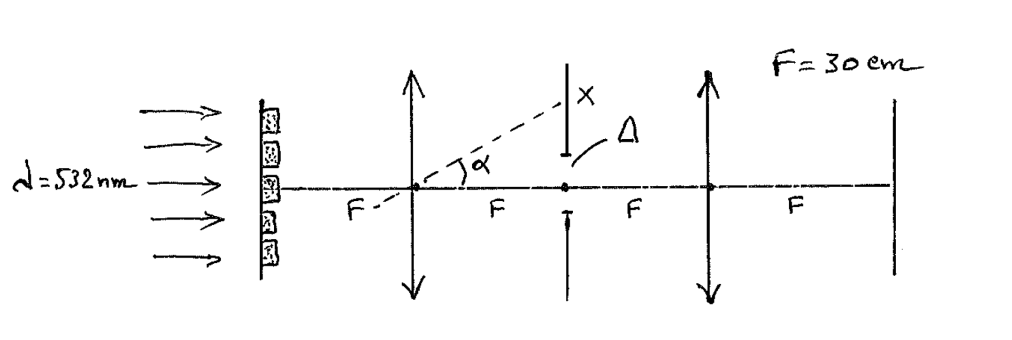
\includegraphics[width=0.8\textwidth]{abbe.png}
\end{figure}

Notion de cohérence temporelle (longueur de cohérence)

\begin{enumerate}
    \item Qu’est-ce ?
    \item De quoi dépend-elle ?
    \item Comment la mesurer ?
\end{enumerate}

\begin{solution}

\begin{enumerate}
    \item $\Delta/2 = f\,\theta$ avec $\theta = \lambda / (2\Lambda)$ le premier zero d'intensité: 
    \[
     \Delta = \frac{f \lambda}{\Lambda} = \SI{1.596}{mm}
    \]
    Ce filtre permet de couper les raies \textbf{horizontales}.
    \item En plus des raies verticales, des raies \textbf{horizontales} apparaissent sur l'écran.
    \item Les couleurs associées à un plus grand angle de premier zéro d'intensité ne subissent pas d'interférence, ce sont les couleurs ayant une longueur d'onde supérieure à 532 nm. C'est donc majoritairement du jaune, orange, rouge.
\end{enumerate}

\end{solution}

\section{Adaptation de la divergence d’un faisceau laser}

\begin{figure}[h!]
    \centering
    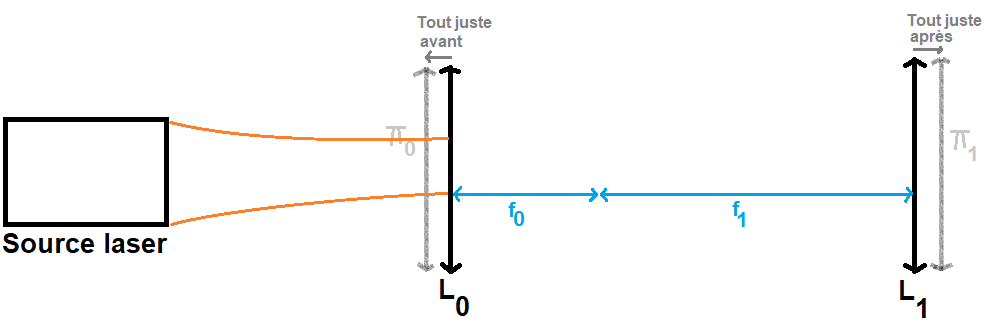
\includegraphics[width=0.7\textwidth]{ex4.png}
    \caption{Montage expérimental}
    \label{ex4}
\end{figure}

Le système décrit par la figure \ref{ex4} est un essai pour réduire la divergence d'un laser. On a le waist $w_0$ à la lentille $L_0$. $z_R$ est donné. La longueur d'onde du laser formé est $\lambda_0 = \SI{532}{nm}$.

\begin{enumerate}
    \item Dans quelle gamme de couleur est le rayon?
    
    \item Exprimer $w_0$ et $\theta$ en fonction de $z_R$.
    
    
    \item Faire l'application numérique pour $z_R = \SI{10}{cm}$.
    
    \item 
    
    \begin{enumerate}
     \item Trouver $T_{\Pi_0 \rightarrow \Pi_1}$, la matrice de transfert. Vérifier que $C=0$ et $A\cdot D$ a la valeur attendue.
     \item Soit $q_0$ et $q_1$ les rayons de courbure complexe en $\Pi_0$ et $\Pi_1$. Exprimer $q_0$ en fonction des données du problème. Exprimer $q_1$ en fonction de $f_0$, $f_1$ et $q_0$, puis ensuite $f_0$, $f_1$ et $z_R$. 
     \item Soit $O"$ la position du waist après transformation par le système optique. Rappeler $q_1(q")$ et $\overline{O"\Omega_1}$. Par identification, donner $z_R"$ et  $\overline{O"\Omega_1}$. Le waist se trouve-t-il à gauche ou à droite de $L_1$?
     \item Exprimer le nouvel angle de divergence. Quelle est la condition pour avoir réduction de la divergence? Quel est le facteur? 
     \item Que peut-on dire du nouveau waist $w_0 "$? 
     \item Bonus : Trouver $f_0$ et $f_1$ pour obtenir un waist de \SI{2.2}{m} après $L_1$ et réduction de 10.
    \end{enumerate}
    
\end{enumerate}

\begin{solution}

\begin{enumerate}
    \item Visible (vert).
    \item $w_0 = \sqrt{\frac{\lambda z_R}{\pi}}$ \hspace{3cm} $\theta = \arctan\left(\sqrt{ \frac{\lambda}{\pi z_R}} \right) \approx \sqrt{ \frac{\lambda}{\pi z_R}}$.
    \item $w_0 = \SI{130}{\micro m}$ et $\theta \approx \SI{1.3e-3}{rad}$.
    \item 
    
    \begin{enumerate}
     \item $T_{\Pi_0 \Rightarrow \Pi_1} = T_{L_1}.T_{propag}.T_{L_0} 
        = \begin{bmatrix} 1 & 0 \\ \frac{-1}{f_1} & 1 \\ \end{bmatrix} 
         \begin{bmatrix} 1 & f_0+f_1 \\ 0 & 1 \\ \end{bmatrix} 
         \begin{bmatrix} 1 & 0 \\ \frac{-1}{f_0} & 1 \\ \end{bmatrix}
        = \begin{bmatrix} \frac{-f_1}{f_0} & f_0+f_1 \\ 0 & \frac{-f_0}{f_1} \\ \end{bmatrix}$\\
        $A\cdot D=1$ comme attendu car correspond au déterminant, et on reste dans le même milieu, il n'y a donc pas de changement d'indice de réfraction. 
     \item $q_0 = i.z_R$. On a $r_i=w_i$ et $\theta_i = \frac{w_i}{q_i}$. On applique la matrice $\begin{bmatrix} w_1  \\ \frac{w_1}{q_1}  \\ \end{bmatrix}
        = T_{\Pi_0 \Rightarrow \Pi_1}.\begin{bmatrix} w_0  \\ \frac{w_0}{q_0}  \\ \end{bmatrix}$.\\ (Ou simplement $q_1=\frac{A\:q_0\:+\:B}{C\:q_0\:+\:D}$).\\
        On trouve $q_1 = \left( \frac{f_1}{f_0} \right)^2q_0 - (f_1+f_0) \frac{f_1}{f_0} = i  \left( \frac{f_1}{f_0} \right)^2z_R -  (f_1+f_0) \frac{f_1}{f_0}$. 
     \item $q_1 = q^" + \overline{O"\Omega_1} \Leftrightarrow q_1 = iz_R^" + \overline{O"\Omega_1} = i  \left( \frac{f_1}{f_0} \right)^2z_R \underbrace{- (f_1+f_0) \frac{f_1}{f_0}}_{<0 \text{ donc $O''$ à droite de } \Omega_1}$ 
     \item $\theta^" = \frac{w_0^"}{z_R^"}=\sqrt{\frac{\lambda}{\pi z_R}}\frac{f_0}{f_1}=\theta\frac{f_0}{f_1}$. La condition pour avoir réduction de divergence est donc $f_1>f_0$.
     \item $|w_0"| = \frac{f_1}{f_0} |w_0|$. Le nouveau waist est plus large. Ce qui est logique car plus un faisceau est large, moins il est divergent.
     \item Bonus: $f_1 = 10 \:f_0$ avec $f_1=\SI{200}{mm}$.
    \end{enumerate}
    
\end{enumerate}

\end{solution}

\end{document}

